\section{Validation}
\label{sec:validation}

Three kinds of oracle are used, and every result says which one it was checked against: QSPICE
golden outputs~\cite{qspice}, committed and gated in continuous integration; closed-form
expressions where no SPICE primitive exists (photonics, sampled systems); and, at scale, the
circuit's Boolean function (Section~\ref{sec:scale}). No golden file is computed by hand.

\begin{table}[t]
  \centering
  \caption{QSPICE golden validation, 28 circuits \src{cargo xtask validate at 2.0.0+2, 2026-09-28}}
  \label{tab:golden}
  \begin{tabular}{@{}llrr@{}}
    \toprule
    Analysis & Metric & Tolerance & Worst error \\
    \midrule
    DC (8)        & max rel.\ I--V error       & $10^{-4}$ & $6.8\times10^{-5}$ \\
    Transient (10)& waveform RMS error         & $10^{-3}$ & $8.3\times10^{-4}$ \\
    AC (5)        & max rel.\ magnitude error  & $10^{-4}$ & $1.3\times10^{-5}$ \\
                  & max abs.\ phase error (rad)& $10^{-4}$ & $6.4\times10^{-6}$ \\
    Noise (5)     & max rel.\ PSD error        & $10^{-3}$ & $2.6\times10^{-5}$ \\
    \bottomrule
  \end{tabular}
\end{table}

\todo{Per-circuit table in an appendix or supplementary material (the 28 rows from
\texttt{xtask validate}). The worst transient case is the diode rectifier, $8.3\times10^{-4}$ against
$10^{-3}$: explain.}

\todo{Jacobian validation against finite differences; count of tests; the workspace test suite
(920 tests at 2.0.0).}

\todo{Closed-form and paper-figure validations outside electronics (photonic noise, thermal,
traffic), from the repository's validation registry, as a short multi-physics subsection or
dropped for length. The micro-ring case study (Section~\ref{sec:mrm}) is the electro-optic one.}

\subsection{Case Study: Silicon Micro-Ring Modulators}
\label{sec:mrm}

The golden circuits above test the simulator against a reference simulator. This case study
tests the claim the tool is built for: that a Verilog-A model written for a commercial or OSDI
flow runs in \vas{} unchanged, with no host simulator and no native compiler, and reproduces the
published results the model was written to reproduce. Two electro-optic micro-ring modulator
(MRM) models were written as ordinary Verilog-A, using only \texttt{ddt}, \texttt{limexp},
\texttt{\$limit} and the standard disciplines, so that the same source compiles with
OpenVAF~\cite{openvaf} for ngspice~\cite{ngspice} through OSDI. Both models share one port list:
the optical field envelope travels on electrical nets in units of $\sqrt{\text{mW}}$ (real and
imaginary parts on two nets), the laser wavelength on a net in nanometres, and the ring
temperature on a \texttt{thermal} node. The ring itself is described by temporal coupled-mode
theory (TCMT), two real ODEs on internal nodes.

\subsubsection{Depletion-mode ring against an OSDI flow}
The first model (\texttt{mrm\_tcmt}) couples a TCMT ring to a lumped p-n junction, a heater and
a thermal node, and is driven by a behavioural two-pole driver at 25\,Gb/s with a PRBS7 sequence
(254 bits). Table~\ref{tab:mrm-tcmt} compares \vas{} with ngspice-47 running the same source
through OpenVAF. The DC spectrum is checked against the closed-form Lorentzian; the transient
power waveform against a tightly converged ngspice run (reltol $10^{-7}$, maximum step 50\,fs),
resampled on a 50\,fs grid. At default settings the two simulators agree with that reference
to the same order, $3.2\times10^{-5}$ and $4.2\times10^{-5}$ RMS of the mean power, and \vas{}
at tight tolerances matches the ngspice reference to $1.5\times10^{-6}$. The same source with
the measured-fit parameters of Saxena and Shawon~\cite{saxena2023mdm} reproduces the resonance
position and depth of their Eq.~(6) exactly over $-0.5$ to 2\,V, with a largest deviation of
$1.2\times10^{-4}$ in transmission in the far skirts, which comes from the FSR-periodic detuning
map used away from resonance.
\src{paper\_writing/mrm\_tcmt/reference/REFERENCE.md and outputs/manifest.json, 2.42.0;
mrm\_tcmt/README.md (Saxena mode 1)}

\begin{table}[t]
  \centering
  \caption{Depletion-mode MRM, 25\,Gb/s PRBS7: \vas{} and ngspice/OpenVAF on the same
  Verilog-A source (2-vCPU x86-64 VM)
  \src{mrm\_tcmt/reference/REFERENCE.md, verilog-a-sim 2.42.0, ngspice-47, 2026-10-23}}
  \label{tab:mrm-tcmt}
  \setlength{\tabcolsep}{4pt}
  \begin{tabular}{@{}lrrr@{}}
    \toprule
    Case & Points & Wall (s) & Error \\
    \midrule
    ngspice DC, default            & \num{2000}   & 0.010 & $2.5\times10^{-5}$ \\
    \vas{} DC, default             & \num{2001}   & 0.14  & $1.2\times10^{-6}$\,$^a$ \\
    ngspice tran, default          & \num{21091}  & 0.18  & $4.2\times10^{-5}$ \\
    \vas{} tran, default           & \num{24650}  & 1.96  & $3.2\times10^{-5}$ \\
    \vas{} tran, default, JIT      & \num{24650}  & 1.72  & identical \\
    ngspice tran, tight (reference)& \num{239343} & 2.34  & --- \\
    \vas{} tran, tight, JIT        & \num{237229} & 45.9  & $1.5\times10^{-6}$ \\
    \bottomrule
    \multicolumn{4}{@{}p{0.95\columnwidth}@{}}{\footnotesize DC error: max.\ $|\Delta T|$
    against the closed form. Transient error: RMS $\Delta P/\bar P$ against the tight ngspice
    run. $^a$\,the print precision of the output (six decimals), not the solver.}
  \end{tabular}
\end{table}

Two further observations follow from this comparison. First, the \vas{} outputs are
bit-identical across machines: re-run on Windows~11 (Intel Core i7-1185G7), the four \vas{} cases
of Table~\ref{tab:mrm-tcmt} reproduce the Linux point counts, step sequence and output hashes
exactly, as Section~\ref{sec:determinism} predicts.
\src{mrm\_tcmt/reference/outputs\_windows, check\_rerun.py, 2.42.0+1, 2026-10-24}
Second, \vas{} is 10 to 20 times slower than the OpenVAF-compiled model in ngspice on this
circuit, and its timing includes parsing and compiling the Verilog-A source on every run.
For a model of this size that is the difference between a fraction of a second and a few
seconds; Section~\ref{sec:limitations} returns to it.

\subsubsection{Reproducing a published carrier-injection model}
The second model (\texttt{mrm\_pin}) is an independent implementation of the compact model of
Wang \emph{et al.}~\cite{wang2016mrm}, a carrier-injection (p-i-n) ring for 1.31\,\textmu m
optical interconnects whose electrical part is Strollo's tenth-order p-i-n
model~\cite{strollo1997pin}. The ring's delayed-feedback equation, Eq.~(4) of~\cite{wang2016mrm},
needs \texttt{absdelay}, which OpenVAF does not support and which \vas{} refuses in transient
analysis; the model therefore uses the equivalent TCMT form, which agrees with Eq.~(4) to
1.7--2.2\,\textmu W RMS on the same carrier waveform. The quantities the paper does not give
were set as follows, and are flagged in the model: the thermal voltage of the junction law is
taken at 58\,$^\circ$C, the only temperature at which the paper's Table~I reproduces its own
I--V curve, and the active carrier volume is calibrated on a single point, the $-90.7$\,pm
resonance shift at 0.86\,V.
\src{paper\_writing/mrm\_injection/README.md}

\begin{figure*}[t]
  \centering
  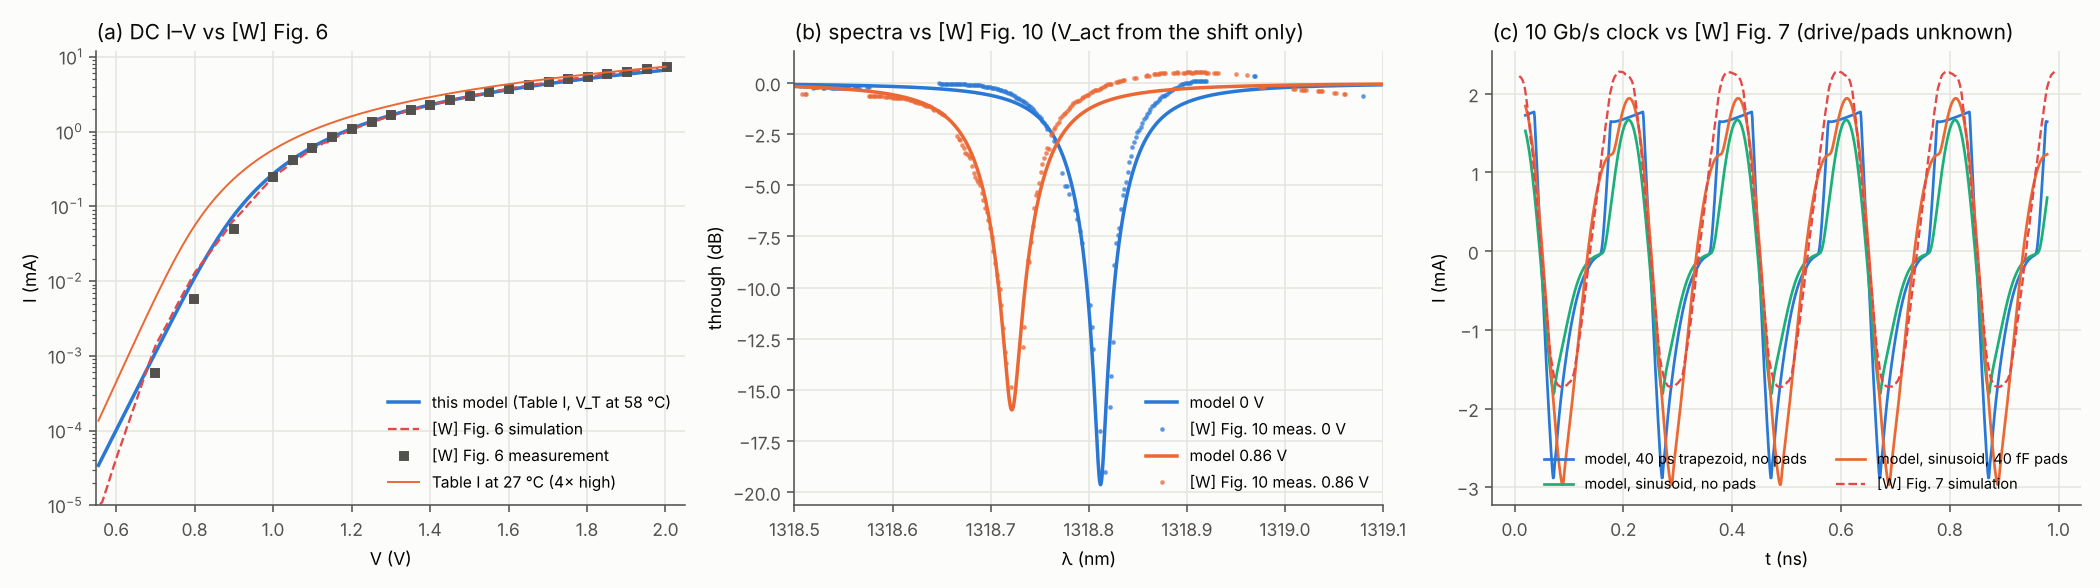
\includegraphics[width=\textwidth]{figures/mrm_pin_static.png}
  \caption{Carrier-injection MRM~\cite{wang2016mrm} in \vas{}. (a) DC I--V against the paper's
  simulation and measurement. (b) Through-port spectra at 0 and 0.86\,V against the measured
  spectra; only the shift at 0.86\,V was used for calibration, not the depth. (c) Current under
  a 10\,Gb/s clock: without the pad and probe parasitics, which the paper does not give, the
  model does not reproduce the paper's near-sinusoidal waveform; adding about 40\,fF of pad
  capacitance and a sinusoidal drive moves it towards it.
  \src{mrm\_injection/tests/plot\_validation.py}}
  \label{fig:mrm-pin-static}
\end{figure*}

The main results of~\cite{wang2016mrm} are reproduced (Fig.~\ref{fig:mrm-pin-static} and
Table~\ref{tab:mrm-pin}). The DC I--V curve lies within 12\,\% RMS of the paper's simulation and
22\,\% of its measurement between 0.66 and 2\,V. The 0\,V spectrum matches the paper's closed form
to $8\times10^{-5}$ in transmission, and the 0.86\,V spectrum, whose depth was not used in the
calibration, reaches $-16.0$\,dB against $-15.4$\,dB simulated and $-14.9$\,dB measured. At
8\,Gb/s, PRBS7, 2\,V$_\text{pp}$, observed through the paper's 20\,GHz Bessel--Thomson receiver,
the model reproduces the central result of the paper (Fig.~\ref{fig:mrm-pin-eyes}): a plain NRZ
drive leaves the eye closed, and pre-emphasis with an 80\,ps pulse opens it to 792\,\textmu W
with a 12.1\,dB extinction ratio. The degradations the paper reports when the emphasis depth is
raised to 0.9\,V or the bias moved to 0.75\,V or 0.65\,V are also reproduced.

\begin{table}[t]
  \centering
  \caption{Carrier-injection MRM at 8\,Gb/s against~\cite{wang2016mrm}: eye height through a
  20\,GHz receiver \src{mrm\_injection/tests/eyes\_va.json, eyes\_ng.json}}
  \label{tab:mrm-pin}
  \setlength{\tabcolsep}{4pt}
  \begin{tabular}{@{}llrc@{}}
    \toprule
    Case in~\cite{wang2016mrm} & Paper & Model (\textmu W) & Agrees \\
    \midrule
    Fig.~12, NRZ, no pre-emphasis   & closed   & closed & yes \\
    Fig.~13(b), 80\,ps pre-emphasis & optimum  & 792    & yes \\
    Fig.~13(a), 40\,ps              & degraded & 844    & no \\
    Fig.~14(a), depth 0.9\,V        & degraded & 292    & yes \\
    Fig.~14(b), depth 0.7\,V        & degraded & 784    & weak \\
    Fig.~15(a), bias 0.75\,V        & degraded & 772    & yes \\
    Fig.~15(b), bias 0.65\,V        & degraded & 702    & yes \\
    Fig.~21(a), asym.\ vs sym.\ (15\,Gb/s) & asym.\ better & 428 vs 467 & no \\
    \bottomrule
  \end{tabular}
\end{table}

\begin{figure*}[t]
  \centering
  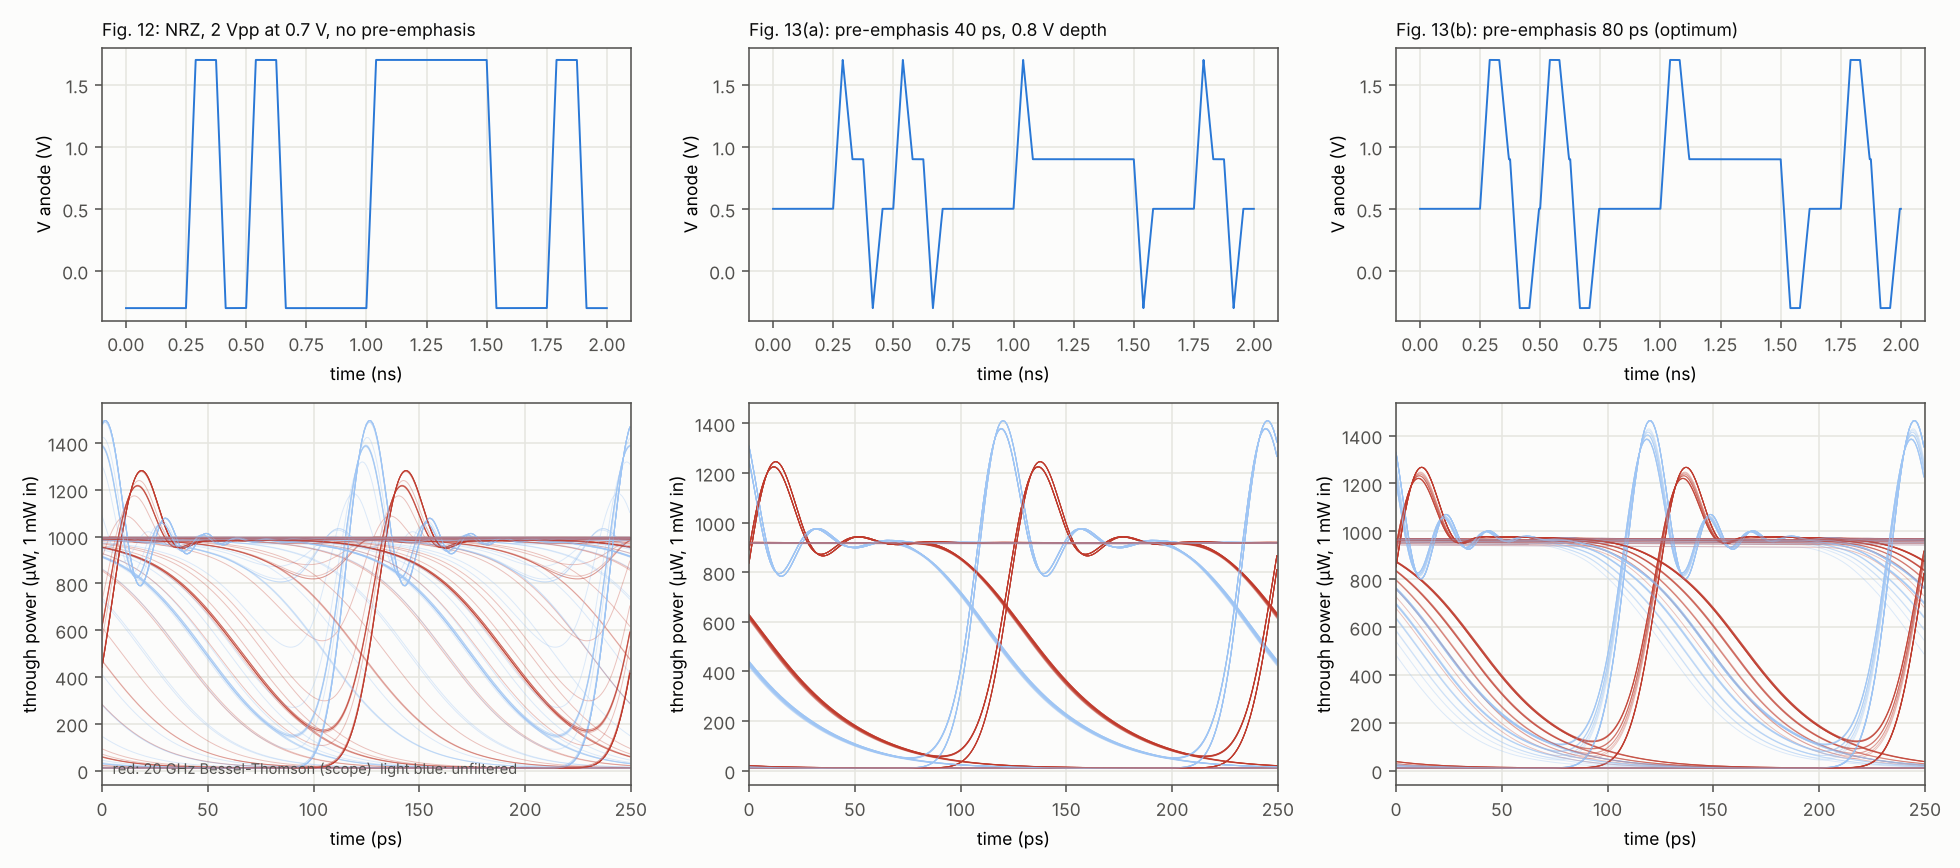
\includegraphics[width=\textwidth]{figures/mrm_pin_eyes.png}
  \caption{Carrier-injection MRM at 8\,Gb/s, PRBS7, laser at the 0\,V resonance: drive
  (top) and optical eye (bottom; red: through the 20\,GHz receiver, light blue: unfiltered) for
  the cases of Figs.~12, 13(a) and 13(b) of~\cite{wang2016mrm}.
  \src{mrm\_injection/tests/plot\_eyes.py va}}
  \label{fig:mrm-pin-eyes}
\end{figure*}

What is not reproduced traces to the measurement setup rather than to the device. The 10\,Gb/s
current waveform of Fig.~7 in~\cite{wang2016mrm} is near-sinusoidal; the model's is not, with
an RMS difference of 0.5--0.75\,mA on $\pm2$\,mA. That waveform depends on elements the paper
does not give, the source impedance, the drive at the probe and the pad and probe parasitics,
and Fig.~\ref{fig:mrm-pin-static}(c) shows that about 40\,fF of pad capacitance alone moves
the model most of the way. Without the pad parasitics of the measured device, the experimental
waveforms cannot be reproduced exactly. Two eye trends are not reproduced either (Fig.~13(a)
and Fig.~21(a)); both have the same signature, a rising edge that depends less on the charge
left by the preceding low level than in the paper. The missing setup parasitics are the first
candidate; a carrier volume calibrated on a single DC point and the depletion capacitance, which
the paper's model omits, are the others, and none of them can be settled from the paper alone.

\subsubsection{Numerical robustness without tuning}
The same nine eye cases run in ngspice through OpenVAF agree with \vas{} to within
0.24\,\textmu W in eye height and 0.01\,dB in extinction ratio. Getting there, however, required
changes for ngspice and none for \vas{}. The direct form of the free-carrier filter contains
two \texttt{ddt} terms of an exponential that cancel analytically. With it, ngspice leaves a
small \emph{negative} free charge after a falling edge, which is unphysical and persists:
0.04\,\% of the peak free-carrier current at reltol $10^{-5}$ and 0.2\,\% at its default
reltol, or 2.6 and 11\,\textmu W on the through power, and at reltol $10^{-5}$ it takes
20\,\% more time steps.
The model was therefore rewritten in an equivalent form without a derivative of the
exponential. The ladder state had
to be scaled to microamperes, because in milliamperes the small shunt nodes sit near ngspice's
default voltage tolerance and Newton stops early. OSDI passes only the global tolerances to the
model, so the discipline \texttt{abstol} could not be used instead. On the 10\,Gb/s terminal
current, the milliampere form is off by 7.7\,\% at ngspice's defaults and the microampere form by
0.87\,\%. The testbenches therefore also need reltol $10^{-5}$, which brings the shipped form to
0.04\,\%. Tightening reltol further is not safe either: at $10^{-9}$ ngspice aborts the
microampere form at the first edge with a timestep collapse to $6\times10^{-25}$\,s.
\src{mrm\_injection/README.md "Numerics": ngspice-47 + OpenVAF on Linux, tb\_fig7.cir, scaling
$\times$ reltol, reference mA at reltol $10^{-9}$, 2026-10-24}
\vas{} gave the correct result with both forms of the model at its default
settings, whose Newton tolerance is $10^{-9}$: on a single pre-emphasis bit the two forms give
the same free-carrier current to $10^{-6}$\,mA, the output's print precision, and neither goes
negative after the fall.
\src{mrm\_injection/README.md "Numerics": ngspice-47 + OpenVAF on Linux, pulse\_ng.cir and
pulse\_direct\_ng.cir, 2026-10-24, data in tests/24-10-4times; tests/fc\_form\_check.py,
verilog-a-sim 2.42.0+5}
On the same 10\,Gb/s current and against the same reference, \vas{} at its defaults is within
0.028\,\% (0.011\,\% RMS), as close as ngspice's tuned setting. Tightening its step control
leaves that at about 0.025\,\%, the level at which the two simulators agree.
\src{mrm\_injection/tests/tolcheck/compare.py --va, verilog-a-sim 2.42.0+13, 2026-10-24}

\subsubsection{An equivalent-circuit ring model, and the simulator as a design tool}
The third package (\texttt{mrm\_eqc}) implements the depletion-ring model of Bao
\emph{et al.}~\cite{bao2024mrm} twice: as its linear RLC equivalent circuit, and as a
large-signal TCMT model with the same parasitics, bias-dependent loss and a thermal node for
heater and self-heating. The two agree to 0.06--0.16\,\% in small-signal response, and the
ngspice and \vas{} eye waveforms agree to $5$--$6\times10^{-5}$ RMS.
\src{mrm\_eqc/README.md sections 1, 3}
The reproduction of~\cite{bao2024mrm} is partial, and the model says where. The resonance
positions match within 0.3\,pm. The dips come out 2--10\,dB too deep, because the paper's
Table~II makes the ring under-coupled, so its dip must deepen with reverse bias while the
measured one shallows. The paper's 32\,GHz electro-optic bandwidth is reached only if its
detunings are read from the cold rather than the heated resonance.
\src{mrm\_eqc/README.md section 2}

The paper reports an open 212\,Gb/s PAM8 eye but not the drive swing, laser power, detuning or
equalisation behind it. With the model running standalone, those unknowns can be searched
directly. That took about 3\,500 transient runs of 8\,000 time points each, at 1.3--1.6\,s per
run with seven runs in parallel on a laptop CPU (i7-1185G7).
\src{mrm\_eqc/tests/t6*.json, t7*.json: run counts and wall times, 2.42.0+7..+9}
Without equalisation no combination opens the eye: the best of 180 drive conditions is $-86$\,\%
of the ideal opening, and a self-heating-free scan of the laser over $\pm1.5$ half-linewidths
finds none open either. The ring's bandwidth closes it, not the drive: the same settings give
$+45$\,\% at a quarter of the symbol rate. A peak-limited three-tap FFE, whose taps keep the
drive inside the same bias window, opens it to $+17$\,\% of ideal. Changing only the bus
coupling of the paper's ring, so that the loaded $Q$ falls from 7\,540 to 3\,600, opens the eye
without any equalisation ($+25$\,\%); with FFE the best ring has $Q_L\approx5\,500$ and reaches
$+37$\,\% (Fig.~\ref{fig:mrm-eqc-eye}). Beyond that point the gain in bandwidth is outweighed by
the loss in modulation depth.
\src{mrm\_eqc/README.md sections 3b, 3c; tests/t6\_pam8\_sweep.py, t7\_lowq\_sweep.py}

\begin{figure}[t]
  \centering
  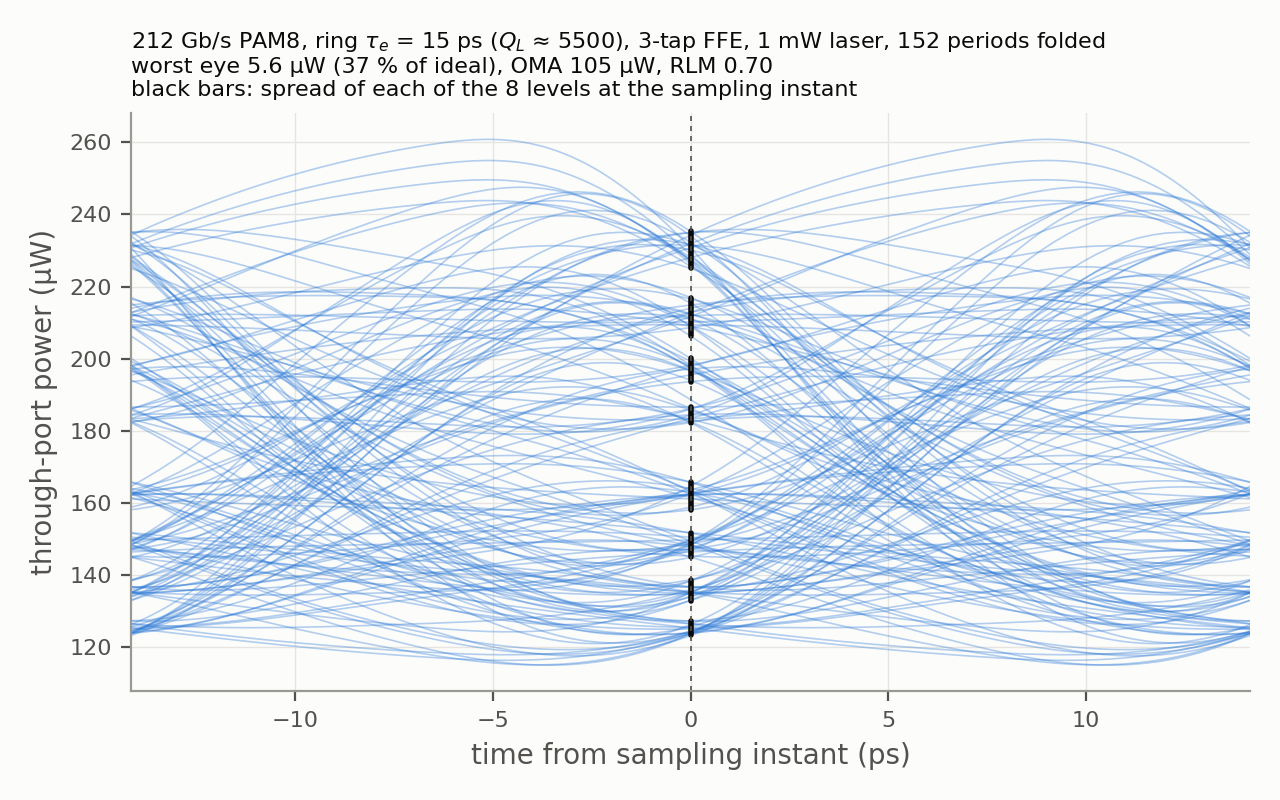
\includegraphics[width=\columnwidth]{figures/mrm_eqc_pam8_eye.png}
  \caption{212\,Gb/s PAM8 eye of the lower-$Q$ variant of the ring of~\cite{bao2024mrm}
  ($\tau_e = 15$\,ps, $Q_L\approx5\,500$; only the bus coupling changed), with a peak-limited
  three-tap FFE and a 1\,mW laser: 152 periods folded, worst eye 5.6\,\textmu W, 37\,\% of
  ideal. \src{mrm\_eqc/tests/t8\_eye\_power.py --eye, 2.42.0+10}}
  \label{fig:mrm-eqc-eye}
\end{figure}

Laser power exposed a numerical trap that is common to every model of this kind, and a way
around it (Fig.~\ref{fig:mrm-eqc-power}). The ring's temperature follows the optical power with
a 1\,\textmu s time constant, so during a 2.4\,ns eye pattern it is frozen at the DC operating
point. Above about 1\,mW the thermal equation of a red-detuned ring has three roots. A DC solve
started cold lands on the cold or the unstable middle root, and a \texttt{.nodeset} on the
thermal node does not move it, because the optical field it would need starts at zero. Direct
self-heating runs therefore showed an apparent collapse of the eye with power that is a
property of the solver's starting point, not of the ring. The frozen temperature is, however,
exactly a laser offset. The eye at any power is then the self-heating-free eye at the same
detuning from the heated resonance, restricted to the detunings that are thermally stable,
$k P\,\mathrm{d}L/\mathrm{d}\delta > -1$, where $L$ is the normalised intracavity power and
$k = 0.215$\,nm/mW. Direct runs at 0.5, 1 and 2\,mW, where the static equation has a single
root, agree with this to 0.5\,\%. The result is that self-heating never closes the eye; it only
moves the best operating point from the red side of the resonance to the blue side above
1.1\,mW, at a cost of 38 to 31\,\% of ideal.
\src{mrm\_eqc/README.md section 3d; docs/frozen-temperature-method.md; t8\_power.json, 2.42.0+11}

\begin{figure*}[t]
  \centering
  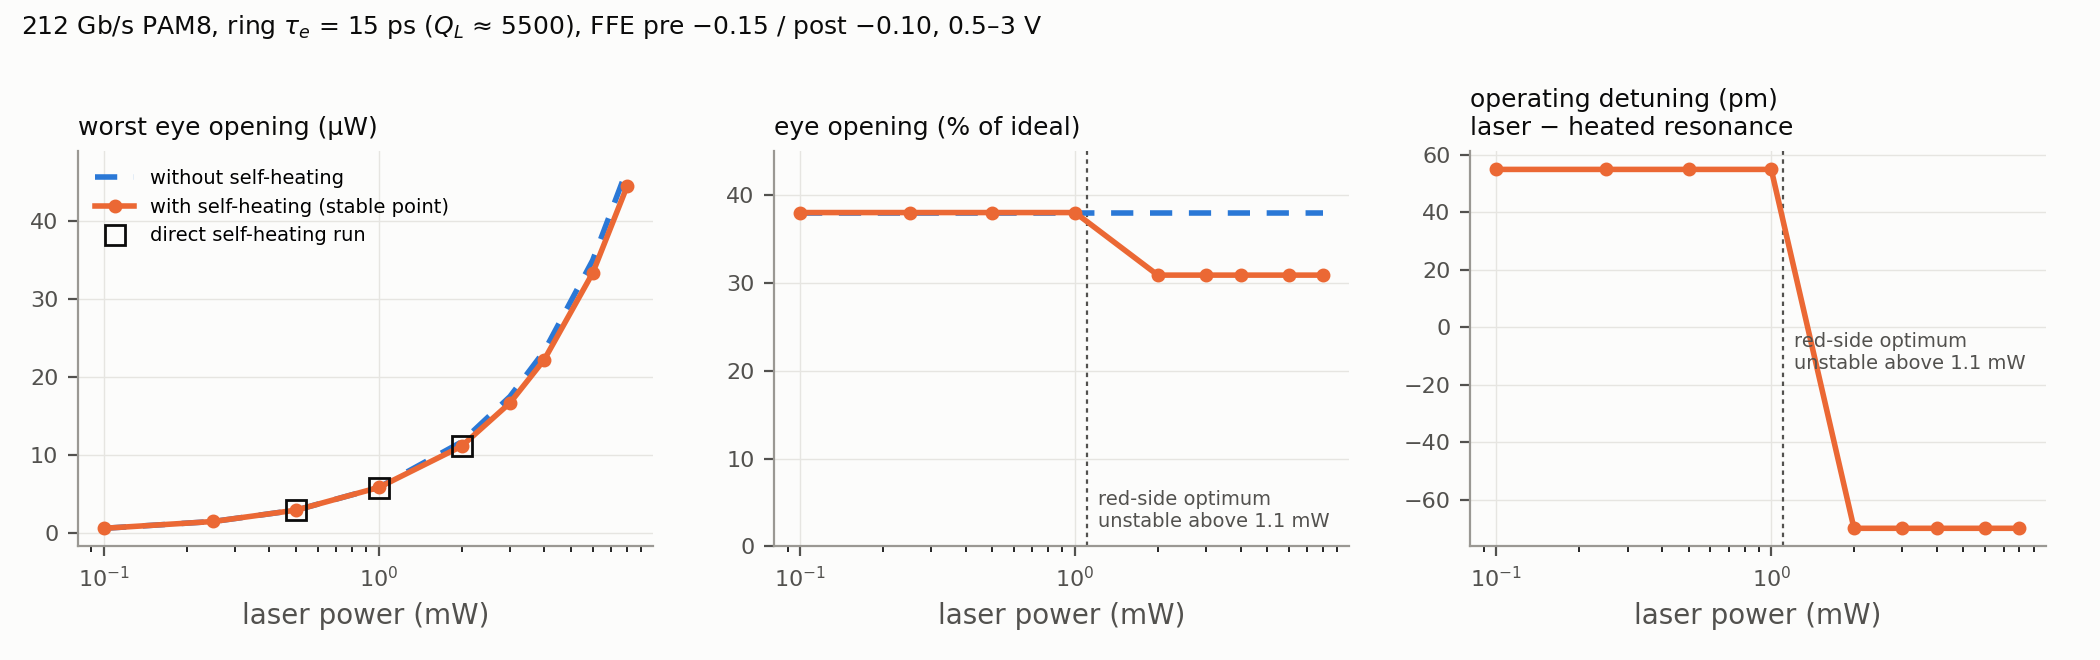
\includegraphics[width=\textwidth]{figures/mrm_eqc_pam8_power.png}
  \caption{Laser power for the ring of Fig.~\ref{fig:mrm-eqc-eye}, with self-heating handled by
  the frozen-temperature method: (left) worst eye opening, (centre) as a fraction of ideal,
  (right) the operating detuning from the heated resonance. The red-side optimum becomes
  thermally unstable above 1.1\,mW. Squares: direct self-heating runs at single-root points.
  \src{mrm\_eqc/tests/t8\_eye\_power.py --power, 2.42.0+11}}
  \label{fig:mrm-eqc-power}
\end{figure*}

The same procedure revisits the package's own PAM4 eyes (Table~\ref{tab:mrm-pam4},
Fig.~\ref{fig:mrm-eqc-pam4}), at 1\,mW with the paper's ring parameters. In the original runs the
laser sat at the wavelength of maximum static OMA. That wavelength came from a static model that
heats each level separately, while the transient kept the first symbol's temperature. Placing
the laser with the frozen-temperature method instead, 80--100\,pm on the blue side of the heated
resonance, roughly doubles the eye height in all four cases. Every point is thermally stable and
confirmed by a direct self-heating run to within 0.2\,\textmu W. Equalisation then matters less
than its usual figure of merit suggests. A peak-limited FFE raises the eye as a fraction of
ideal, for example from 71 to 83\,\% for single-segment 80\,Gb/s, but it does so by giving up
swing. Ranked by eye height, which is what a receiver sees, it helps only the dual-segment
106\,Gb/s case (+14\,\%).
\src{mrm\_eqc/README.md section 3e; tests/t9\_pam4\_ffe.json, t9\_pam4\_height.json, 2.42.0+11}

\begin{table}[t]
  \centering
  \caption{PAM4 on the ring of~\cite{bao2024mrm}, 1\,mW: worst eye height (\textmu W) and
  fraction of ideal \src{mrm\_eqc/tests/t5\_eyes.json, t9\_pam4\_height.json}}
  \label{tab:mrm-pam4}
  \setlength{\tabcolsep}{3pt}
  \begin{tabular}{@{}lrrr@{}}
    \toprule
    Case & Max.\ static OMA & Best placement & + FFE \\
    \midrule
    single, 80\,Gb/s  & 28.7 (53\,\%) & 60.2 (71\,\%) & 60.9 (77\,\%) \\
    dual, 80\,Gb/s    & 24.6 (42\,\%) & 51.6 (54\,\%) & = \\
    single, 106\,Gb/s & 17.8 (31\,\%) & 39.8 (51\,\%) & = \\
    dual, 106\,Gb/s   & 11.2 (17\,\%) & 27.9 (33\,\%) & 31.7 (39\,\%) \\
    \bottomrule
    \multicolumn{4}{@{}p{0.95\columnwidth}@{}}{\footnotesize ``+ FFE'': the taps that maximise
    the eye height; ``='': no taps do better than none.}
  \end{tabular}
\end{table}

\begin{figure*}[t]
  \centering
  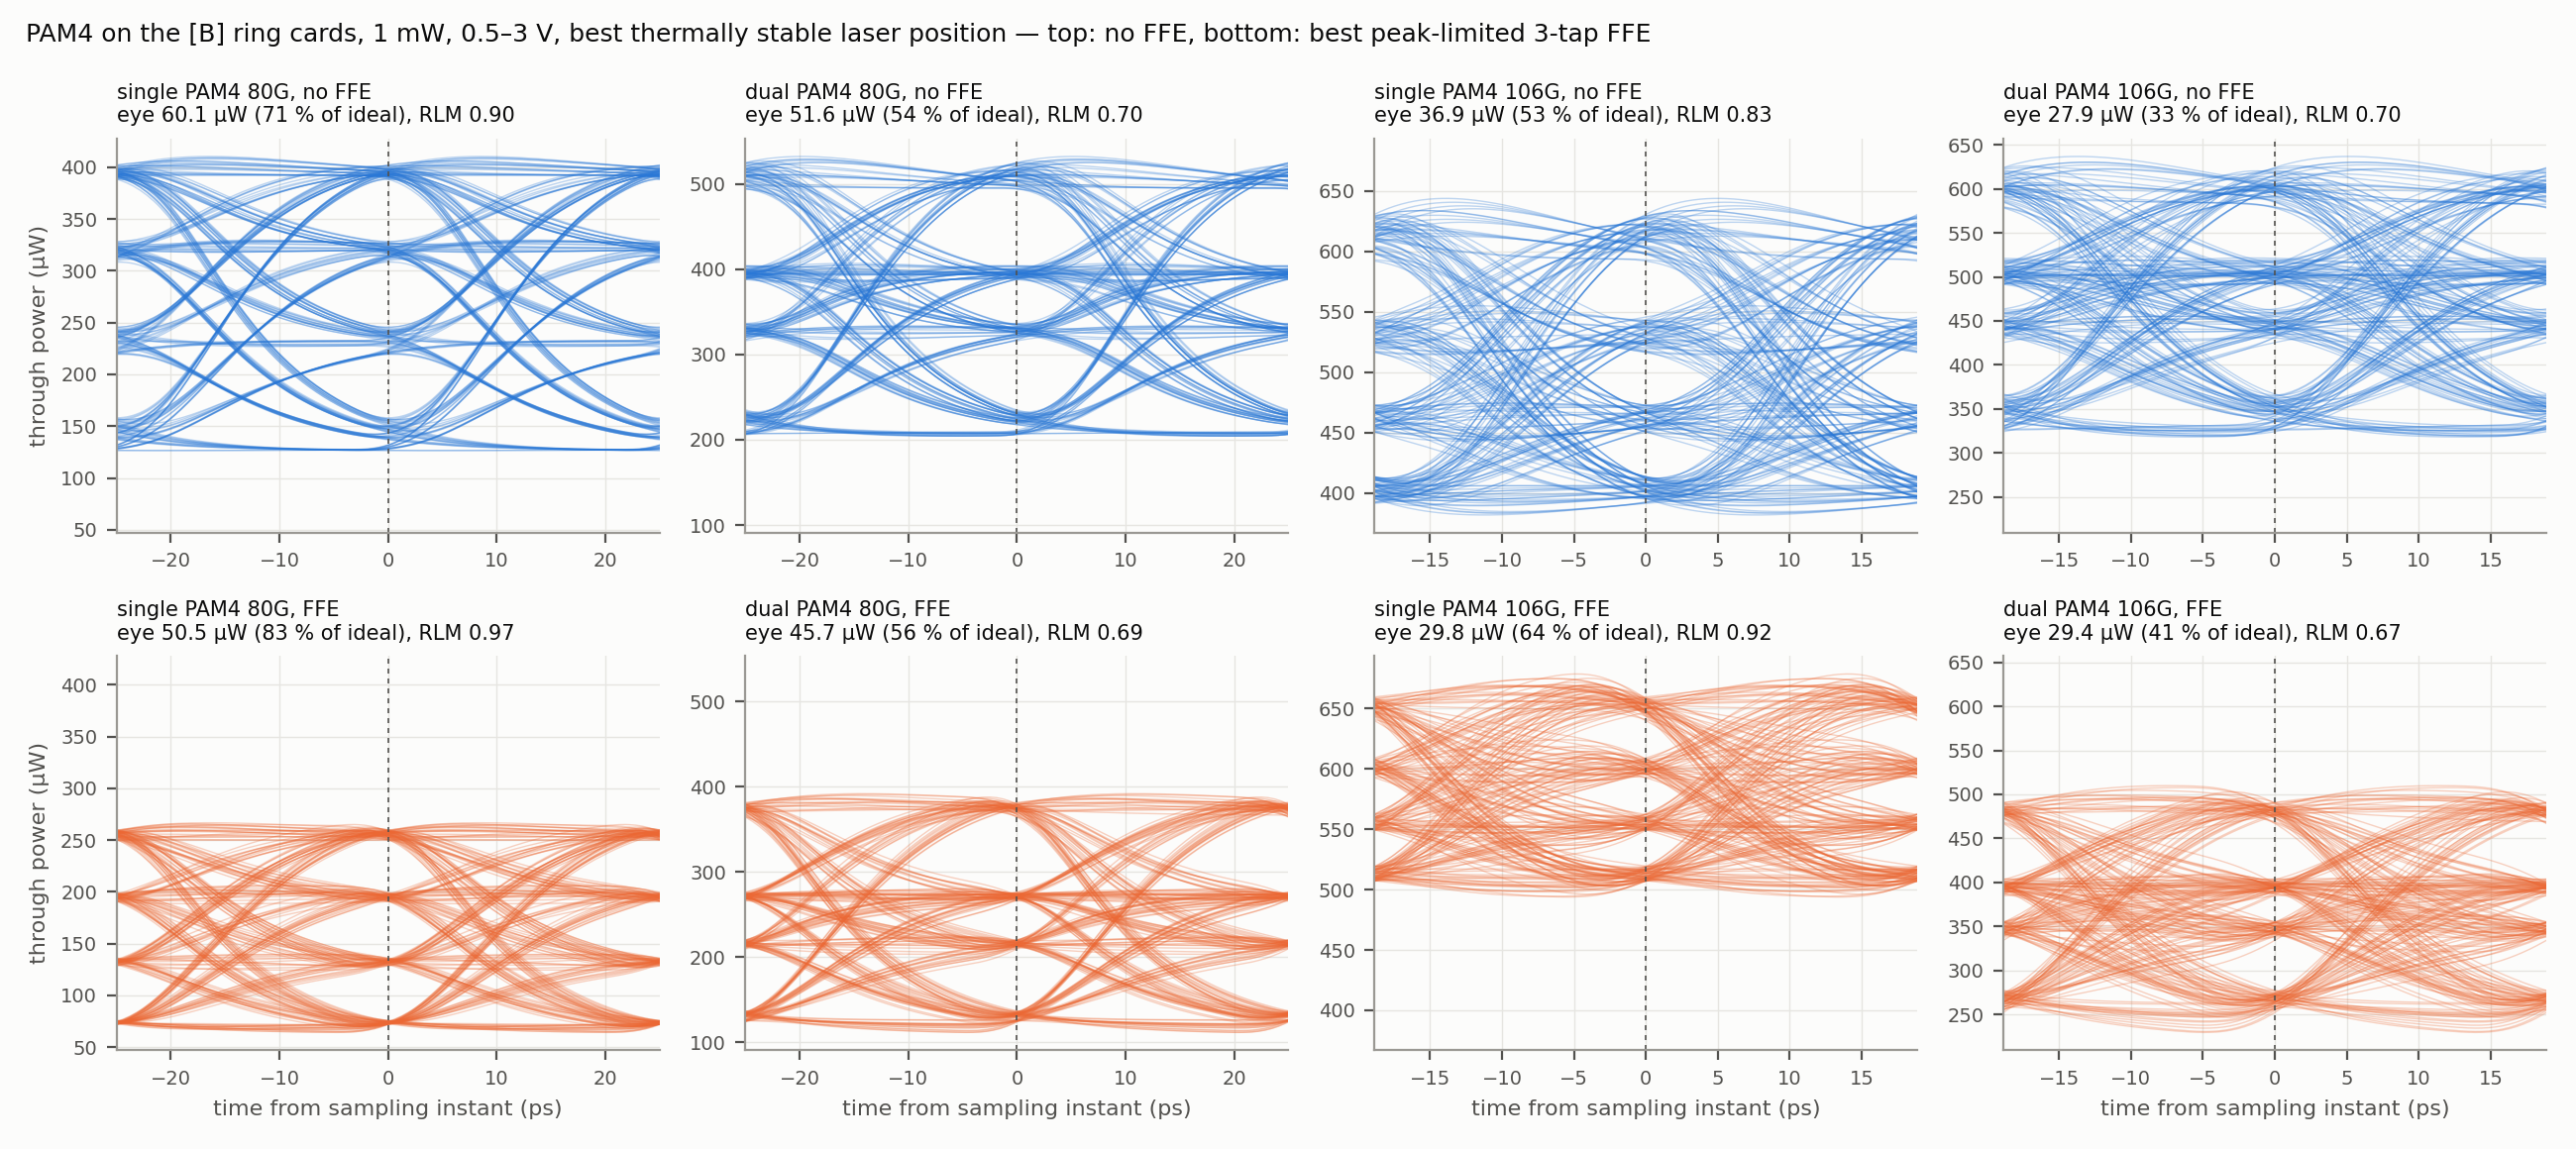
\includegraphics[width=\textwidth]{figures/mrm_eqc_pam4_eyes.png}
  \caption{PAM4 eyes on the ring of~\cite{bao2024mrm} at 1\,mW, laser at the best thermally
  stable position: (top) without FFE, (bottom) with the taps that maximise the eye as a fraction
  of ideal. Those taps flatten the eye at the cost of height, so they are not the height
  optimum of Table~\ref{tab:mrm-pam4}. \src{mrm\_eqc/tests/t9\_pam4\_ffe.py, 2.42.0+11}}
  \label{fig:mrm-eqc-pam4}
\end{figure*}

